%La comunicación entre la PC y el FPGA se realiza mediante tres bloques, los que se pueden apreciar en la Figura \ref{fig:etp}: la comunicación entre el FPGA y la interfaz, la configuración de la interfaz misma y la conexión entre la PC y la interfaz. El desarrollo de cada etapa cuenta con herramientas específicas que facilitan en gran medida la tarea que se realiza. En este capítulo se detalla por separado las características de cada una de estas herramientas.
%Se puede descomponer la implementación en tres partes bien definidas: La comunicación entre el FPGA y la interfaz intermedia, la configuración de la interfaz misma, y la conexión entre la PC y la interfaz. El desarrollo de cada una de estas etapas contará con herramientas específicas.\\

%\begin{figure}
%	\centering
%	\begin{tikzpicture}[]
%	\begin{scope}[transform shape,node distance=1,>=latex]
%	\node[rectangle, rounded corners,draw=black,minimum size=40](memo){Memoria};
%	\node[](aux01)[right=of memo]{};
%	\node[align=center,](comFIFO)[above=of aux01]{Comunicacion\\Interfaz - FPGA};
%	\node[exterior](fpga)[right=of aux01]{FPGA};
%	\node[rectangle, rounded corners, draw=black, minimum size=40,align=center](trans)[left=of memo]{Transceptor\\USB};
%	\node[node distance=.5](aux02)[left=of memo]{};
%	\node[](interfaz)[below=of aux02]{Interfaz};
%	\node[](aux03)[left=of trans]{};
%	\node[align=center](comPC)[above=of aux03]{Comunicación\\PC - Interfaz};
%	\node[exterior](pc)[left=of aux03]{PC};
%	\draw[thick,<->] (fpga) to (memo);
%	\draw[thick,<->] (pc) to (trans);
%	\end{scope}
%	\begin{scope}[]
%	\node[rectangle, dashed, draw=black, rounded corners, fit={(fpga)(memo)(comFIFO)}] (parte1) {};
%	\node[exterior,fit={(trans)(interfaz)(memo)}](bridge){};
%	\node[rectangle, rounded corners, dashed,draw=black, fit={(trans)(pc)(comPC)}](parte3){};
%	\node[rectangle, rounded corners, dashed,draw=black, fit={(interfaz)(bridge)}](){};
%	\end{scope}
%	\end{tikzpicture}
%	\caption{Partes en que se desglosa el trabajo}
%	\label{fig:etp}
%\end{figure}


La parte central del sistema desarrollado en el presente trabajo está constituida por el módulo de interfaz entre el FPGA y la PC. La función de este módulo es comunicarse con una PC a través del protocolo USB 2.0, decodificando los paquetes que recibe la interfaz FX2LP, comprobando que dichos paquetes no contengan errores, separando la información del protocolo USB (encabezado y cola), de la que es útil para el sistema implementado en un FPGA. Además, debe escribir los datos recibidos desde la PC en el FPGA con un protocolo más simple, con el objetivo de utilizar menos recursos programables de este último dispositivo. También debe efectuar el camino inverso de comunicación, es decir leer datos del FPGA, colocar la información que requiere el protocolo y transmitir los paquetes hacia la PC.%\\

En el mercado de componentes electrónicos, existen dos fabricantes que ofrecen interfaces USB (también llamadas puentes USB). Las empresas FTDI y Cypress Semiconductor exhiben en sus catálogos, sendas líneas de productos que proveen circuitos integrados que podrían servir a los fines del desarrollo buscado. Durante la elaboración de este trabajo, se evaluó la alternativa que más se ajusta a las necesidades del sistema desarrollado que brinda cada uno de estos proveedores.

El chip FT4222H de FTDI es un puente USB relativamente simple de configurar, ya que no es necesario elaborar software adicional para que ejecute las tareas relativas a la comunicación. Hacia el lado de los periféricos, la comunicación se realiza mediante el protocolo SPI, con un reloj de hasta \SI{30}{\mega\hertz}. Es posible alcanzar la velocidad máxima permitida por el protocolo USB mediante el uso de cuatro puertos SPI.%Sin embargo, posee una desventaja importante con respecto a los objetivos del presente trabajo. La interfaz de FTDI se comunica con los periféricos que necesitan enviar datos a través de él por un puerto SPI, cuya tasa máxima de transferencia de \SI{53.8}{\mega\bit\per\second}~\cite{FutureTechnologyDevicesInternationalLtd}. Esta característica hace que no sea apropiada para el sistema que se desarrolla.

Por su parte, la línea de circuitos integrados FX2/FX2LP de Cypress Semiconductor ofrece controladores USB muy versátiles y potentes. Los puentes USB poseen, cómo interfaz hacia los periféricos, un conjunto de memorias FIFO a las que se puede acceder por un puerto paralelo de 16 bits de ancho de bus, que pueden operar a 48 MHz. También incorporan un microcontrolador 8051, el cual implementa niveles superiores del protocolo USB, ejecutando las tareas de configuración y control que solicita el Host \cite{CypressSemiconductor2014fx2lp}, y a su vez, puede ser utilizado por el usuario para implementar sistemas adicionales.

Se escoge entonces, para el desarrollo del sistema de comunicación, el controlador FX2/FX2LP de Cypress en lugar de la interfaz fabricada por FTDI ya que el uso de un puerto cuádruple SPI supone una implementación un poco más costosa, en términos de lógica programable, que la comunicación de un puerto paralelo de 16 bits.

Cypress comercializa un kit de desarrollo destinado al diseño de sistemas basados en la serie de controladores FX2LP. Dicho kit de desarrollo se denomina CY3684 EZ-USB FX2LP. El kit posee una placa de desarrollo como la que se observa en la Figura \ref{fig:cy3684}. El componente principal del kit es el controlador EZ-USB FX2LP e incorpora un display de 7 segmentos, 4 luces led multipropósito, 6 pulsadores, de los cuales 4 son de propósito general, uno de reinicio y otro que envía una señal especial para salir de un modo de bajo consumo. También tiene dos memorias EEPROM destinadas al almacenamiento del firmware (programa que ejecuta un microcontrolador), posibilitando la carga no volátil de la configuración del controlador; una memoria Flash con una capacidad de \SI{64}{\kilo\byte} que es utilizada durante la ejecución del firmware, un puerto USB y dos UART con conectores DE-9. Adicionalmente, cuenta con 6 puertos de 20 pines, compatibles con Analizadores Lógicos estándar y un puerto con 40 pines, compatible con el protocolo ATA, que permiten comunicarse con el controlador.
 
%El controlador EZ-USB FX2LP fabricado por Cypress Semiconductor, un circuito integrado que posee en su interior una versión del microcontrolador ($\mu$C) Intel 8051, con algunas mejoras destinadas a satisfacer mejor los requerimientos del sistema USB; una interfaz que permite ingresar datos en serie y los entrega en forma paralela y viceversa; un transceptor USB encargado de todas las tareas de codificación y decodificación de paquetes USB; memoria RAM para programas y datos de \SI{16}{\kilo\byte}. Posee, a su vez, tres tipos de interfaces hacia periféricos externos: I$^2$C, una memoria FIFO (Primero Entrado, Primero Salido, del inglés{\it First In First Out}) destinada a sistemas que pueden comandar la lectura y escritura de datos, y un sistema de propósito general que puede ser comandado a través del $\mu$C 8051~\cite{CypressSemiconductor2014fx2lp}.%\\%a través del cual efectua las tareas que requiere la comunicación USB, sumado a un transceptor USB, el cual codifica y decodifica los paquetes USB que se transmiten a través del bus. A su vez, posee ciertos periféricos e interfaces que otorgan flexibilidad suficiente para adecuar el chip a los requerimientos de un desarrollo determinado.\\

%El controlador viene montado en un circuito impreso que posee una serie de componentes adicionales que facilitan la interacción del desarrollador, tales como pulsadores, display de 7 segmentos, módulos de memoria adicional,etc. Este tipo de circuitos impresos armados con la intención de favorecer desarrollo de otros sistemas, se denomina placa de desarrollo. Una placa de desarrollo que, además, incorpora algunas herramientas extra como software, cables de conexión, fuentes, etc. toma el nombre de kit de desarrollo.%\\

\begin{figure}[ht]
\centering
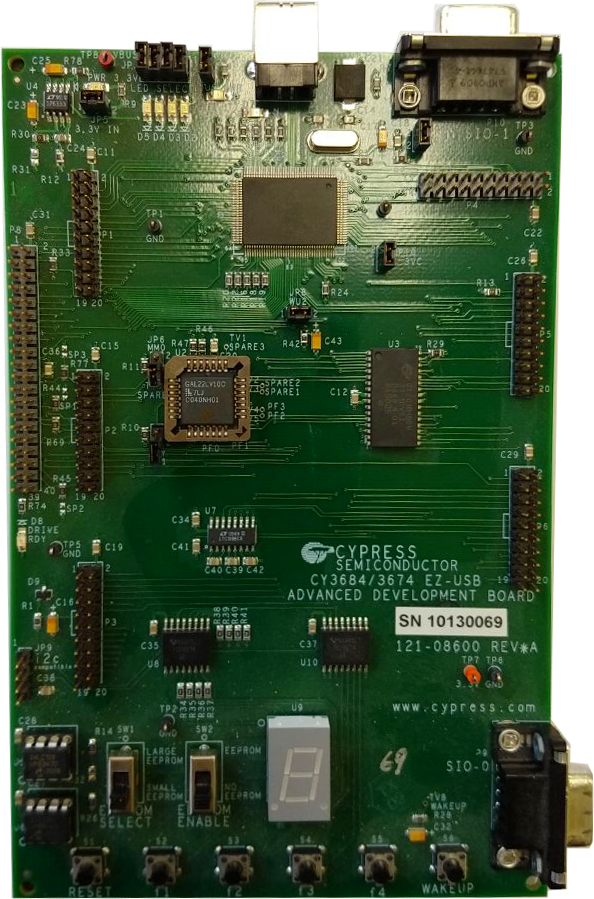
\includegraphics[width=0.4\textwidth]{32cypressboard}
\caption{Circuito impreso principal del kit de desarrollo CY3684 EZ-USB FX2LP}
\label{fig:cy3684}
\end{figure}

%En este trabajo, se utiliza el kit de desarrollo CY 3684 EZ-USB FX2LP, fabricado por Cypress Semiconductor~\cite{CypressSemiconductor2014cy3684}. El kit posee una placa de desarrollo como la que se observa en la Figura \ref{fig:cy3684}. El componente principal del kit es el controlador EZ-USB FX2LP e incorpora un display de 7 segmentos, 4 luces led multipropósito, 6 pulsadores, de los cuales 4 son de propósito general, uno de reinicio y otro que envía una señal especial para salir de un modo de bajo consumo. También tiene dos bloques de memorias EEPROM destinadas al almacenamiento del firmware (programa que ejecuta un microcontrolador), lo que otorga la posibilidad de realizar una carga no volátil de la configuración del controlador, memoria flash de \SI{64}{\kilo\byte} utilizados como RAM por el programa del controlador, un puerto USB y dos puertos UART con zócalos DE-9. Adicionalmente, cuenta con 6 puertos de 20 pines que permiten comunicarse con el controlador y 1 puerto de 40 pines, compatible con el protocolo ATA.%\\
%AQUI QUEDE

%	La arquitectura del controlador EZ-USB FX2LP se muestra en la Figura %TODO la arquitectura, pavo
%	. En ella se puede apreciar los diferentes componentes que se integran en él. Como se menciona anteriormente, la serie de circuitos integrados EZ-USB FX2LP incorporan un microcontrolador 8051, con algunas mejoras destinadas a satisfacer mejor los requerimientos del sistema USB; una interfaz serie, que permite ingresar datos uno tras otro y los entrega en forma paralela y viceversa; un transceptor USB encargado de todas las tareas de codificación y decodificación de paquetes USB; memoria RAM para programas y datos de \SI{16}{\kilo\byte}. Posee, a su vez, tres tipos de interfaces hacia periféricos externos


%	Como interfaz entre la FPGA y la PC se utilizó kit de de desarrollo CY3684 FX2LP EZ-USB Development Kit de Cypress Semiconductor,la que se observa en la Figura \ref{cy3684}. Esta placa posee como núcleo el controlador USB CY7C68013A, circuito integrado que posee todas las herramientas necesarias para realizar la interfaz, como así también un buen número de periféricos que permiten al desarrollador realizar pruebas y depuración.\\


%	Entre estas, se destacan 6 pulsadores, de los cuales cuatro se utilizan para proposito general, uno para reestablecer los valores por defecto de la placa y uno para enviar señales de suspensión y reestablecimiento del programa actualmente cargado en el microcontrolador, lo que coloca al sistema en modo bajo consumo de energía. A su vez, posee dos memorias EEPROM que sirven para cargar firmware y archivos de configuración del sistema, un display de 8 segmentos, 4 leds de multiple propósito, dos puertos UART, una salida de pines compatible con puertos ATA y 6 puertos de 20 pines que se utilizan para la conexión hacia el chip núcleo. Como soporte para el firmware, posee también un bloque con \SI{64}{\kilo\byte} de memoria SRAM.\\

%Se selecciona este controlador como interfaz ya que cuenta con una gran cantidad de herramientas que permiten realizar la comunicación USB, además de poseer memoria suficiente para datos y una interfaz de comunicación para periféricos simple lo que facilita el objetivo de utilizar la menor cantidad de los recursos configurables del FPGA, de forma tal que queden, estos últimos, disponibles para el desarrollo de otros sistemas.%\\
